% !TeX TXS-program:compile = txs:///lualatex

\documentclass[tikz]{standalone}
\usepackage{fontspec}
\setmainfont{DejaVuSansCondensed-Bold.ttf}
\usepackage{customenvs-macros}
\newcommand\positionneHG[2][0,1.125]{%
	\draw (#1) node[below right,font=\scriptsize] {\vphantom{1,2,3,4,5,6,7,8,9,0,°,+,¨,£,µ,\%,?,.,/,§}\halignnb[1,2,3,4,5,6,7,8,9,0,°,+,¨,£,µ,\%,?,.,/,§]{#2}} ;
}
\newcommand\positionneBD[2][1.125,0]{%
	\draw (#1) node[above left,font=\scriptsize] {\vphantom{\textasciitilde,\# ,\{,[,|,`,\textbackslash,\^,@,],\},¤,€}\halignnb[\textasciitilde,\# ,\{,[,|,`,\textbackslash,\^,@,],\},¤,€]{#2}} ;
}

\def\strutletters{0123456789AZERTYUIOPQSDFGHJKLMWXCVBN}

\begin{document}

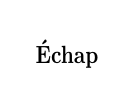
\begin{tikzpicture}%touche échap
	\path (0,0) rectangle (1,0.666);
	\clip (0,0) rectangle (1,0.666);
	\draw (0.5,0.333) node[font=\small\bfseries,xscale=0.8] {Échap} ;
\end{tikzpicture}

\foreach \i in {1,...,12}{%
	\begin{tikzpicture}%Fi
		\path (0,0) rectangle (1,0.666);
		\clip (0,0) rectangle (1,0.666);
		\draw (0.5,0.333) node[font=\small\bfseries] {\vphantom{0123456789}F\i} ;
	\end{tikzpicture}
}


\begin{tikzpicture}%Impréc
	\path (0,0) rectangle (1,0.666);
	\clip (0,0) rectangle (1,0.666);
	\draw (0.5,0.333) node[font=\small\bfseries,xscale=0.65] {Imprécr} ;
\end{tikzpicture}


\begin{tikzpicture}%Inser
	\path (0,0) rectangle (1,0.666);
	\clip (0,0) rectangle (1,0.666);
	\draw (0.5,0.333) node[font=\small\bfseries,xscale=0.9] {\vphantom{p}Inser} ;
\end{tikzpicture}


\begin{tikzpicture}%Suppr
	\path (0,0) rectangle (1,0.666);
	\clip (0,0) rectangle (1,0.666);
	\draw (0.5,0.333) node[font=\small\bfseries,xscale=0.8] {Suppr} ;
\end{tikzpicture}

\begin{tikzpicture}%dots
	\path (0,0) rectangle (1,0.666);
	\clip (0,0) rectangle (1,0.666);
	\draw (0.5,0.333) node[font=\small\bfseries] {*} ;
\end{tikzpicture}

\begin{tikzpicture}%slash
	\path (0,0) rectangle (1,0.666);
	\clip (0,0) rectangle (1,0.666);
	\draw (0.5,0.333) node[font=\small\bfseries] {/} ;
\end{tikzpicture}

\begin{tikzpicture}%carré
	\path (0,0) rectangle (0.75,1.125);
	\clip (0,0) rectangle (0.75,1.125);
	\draw (0.375,0.5625) node[font=\small\bfseries] {{}\textup{2}} ;
\end{tikzpicture}

\begin{tikzpicture}%esper
	\path (0,0) rectangle (1.125,1.125);
	\clip (0,0) rectangle (1.125,1.125);
	\draw (0.5625,0.5625) node[font=\large\bfseries] {\&} ;
%	\positionneHG{1}
\end{tikzpicture}

\begin{tikzpicture}%é
	\path (0,0) rectangle (1.125,1.125);
	\clip (0,0) rectangle (1.125,1.125);
	\draw (0.5625,0.5625) node[font=\large\bfseries] {é} ;
%	\positionneHG{2}
%	\positionneBD{\textasciitilde}
\end{tikzpicture}

\begin{tikzpicture}%é
	\path (0,0) rectangle (1.125,1.125);
	\clip (0,0) rectangle (1.125,1.125);
	\draw (0.5625,0.5625) node[font=\large\bfseries] {"} ;
%	\positionneHG{3}
%	\positionneBD{\#}
\end{tikzpicture}

\begin{tikzpicture}%é
	\path (0,0) rectangle (1.125,1.125);
	\clip (0,0) rectangle (1.125,1.125);
	\draw (0.5625,0.5625) node[font=\large\bfseries] {'} ;
%	\positionneHG{4}
%	\positionneBD{\{}
\end{tikzpicture}

\begin{tikzpicture}%
	\path (0,0) rectangle (1.125,1.125);
	\clip (0,0) rectangle (1.125,1.125);
	\draw (0.5625,0.5625) node[font=\large\bfseries] {(} ;
%	\positionneHG{5}
%	\positionneBD{[}
\end{tikzpicture}

\begin{tikzpicture}%
	\path (0,0) rectangle (1.125,1.125);
	\clip (0,0) rectangle (1.125,1.125);
	\draw (0.5625,0.5625) node[font=\large\bfseries] {-} ;
%	\positionneHG{6}
%	\positionneBD{|}
\end{tikzpicture}

\begin{tikzpicture}%
	\path (0,0) rectangle (1.125,1.125);
	\clip (0,0) rectangle (1.125,1.125);
	\draw (0.5625,0.5625) node[font=\large\bfseries] {è} ;
%	\positionneHG{7}
%	\positionneBD{`}
\end{tikzpicture}

\begin{tikzpicture}%
	\path (0,0) rectangle (1.125,1.125);
	\clip (0,0) rectangle (1.125,1.125);
	\draw (0.5625,0.5625) node[font=\large\bfseries] {---} ;
%	\positionneHG{8}
%	\positionneBD{\textbackslash}
\end{tikzpicture}

\begin{tikzpicture}%
	\path (0,0) rectangle (1.125,1.125);
	\clip (0,0) rectangle (1.125,1.125);
	\draw (0.5625,0.5625) node[font=\large\bfseries] {ç} ;
%	\positionneHG{9}
%	\positionneBD{∧}
\end{tikzpicture}

\begin{tikzpicture}%
	\path (0,0) rectangle (1.125,1.125);
	\clip (0,0) rectangle (1.125,1.125);
	\draw (0.5625,0.5625) node[font=\large\bfseries] {à} ;
%	\positionneHG{0}
%	\positionneBD{@}
\end{tikzpicture}

\begin{tikzpicture}%
	\path (0,0) rectangle (1.125,1.125);
	\clip (0,0) rectangle (1.125,1.125);
	\draw (0.5625,0.5625) node[font=\large\bfseries] {)} ;
%	\positionneHG{°}
%	\positionneBD{]}
\end{tikzpicture}

\begin{tikzpicture}%
	\path (0,0) rectangle (1.125,1.125);
	\clip (0,0) rectangle (1.125,1.125);
	\draw (0.5625,0.5625) node[font=\large\bfseries] {=} ;
%	\positionneHG{+}
%	\positionneBD{\}}
\end{tikzpicture}

\begin{tikzpicture}%
	\path (0,0) rectangle (1.125,1.125);
	\clip (0,0) rectangle (1.125,1.125);
	\draw (0.5625,0.5625) node[font=\large\bfseries] {⟵} ;
\end{tikzpicture}

\begin{tikzpicture}%
	\path (0,0) rectangle (1,1.125);
	\clip (0,0) rectangle (1,1.125);
	\draw (0.5,0.5625) node[font=\large\bfseries] {+} ;
\end{tikzpicture}

\begin{tikzpicture}%
	\path (0,0) rectangle (1,1.125);
	\clip (0,0) rectangle (1,1.125);
	\draw (0.5,0.5625) node[font=\large\bfseries] {--} ;
\end{tikzpicture}


\begin{tikzpicture}%
	\path (0,0) rectangle (1,1.125);
	\clip (0,0) rectangle (1,1.125);
	\draw (0.5,0.5625) node[font=\large\bfseries,xscale=0.5] {Num\,Lk} ;
\end{tikzpicture}

\begin{tikzpicture}%
	\path (0,0) rectangle (1.51,1.125);
	\clip (0,0) rectangle (1.51,1.125);
	\draw (0.755,0.5625) node[font=\large\bfseries] {Tab\,↹} ;
\end{tikzpicture}

\foreach \i in {A,Z,E,R,T,Y,U,I,O,P}{%
	\begin{tikzpicture}%
		\path (0,0) rectangle (1.125,1.125);
		\clip (0,0) rectangle (1.125,1.125);
		\draw (0.5625,0.5625) node[font=\large\bfseries] {\i} ;
%		\ifthenelse{\equal{\i}{E}}{\positionneBD{€}}{}
	\end{tikzpicture}
}

\begin{tikzpicture}%
	\path (0,0) rectangle (1.125,1.125);
	\clip (0,0) rectangle (1.125,1.125);
	\draw (0.5625,0.5625) node[font=\large\bfseries] {∧} ;
%	\positionneHG{¨}
\end{tikzpicture}

\begin{tikzpicture}%
	\path (0,0) rectangle (1.125,1.125);
	\clip (0,0) rectangle (1.125,1.125);
	\draw (0.5625,0.5625) node[font=\large\bfseries] {\$} ;
%	\positionneHG{£}
%	\positionneBD{¤}
\end{tikzpicture}

\begin{tikzpicture}%
	\path (0,0) rectangle (1.125,1.125);
	\clip (0,0) rectangle (1.125,1.125);
	\draw (0.5625,0.5625) node[font=\large\bfseries] {*} ;
%	\positionneHG{µ}
\end{tikzpicture}

\foreach \i in {7,8,9}{%
	\begin{tikzpicture}%
		\path (0,0) rectangle (1,1.125);
		\clip (0,0) rectangle (1,1.125);
		\draw (0.5,0.5625) node[font=\large\bfseries] {\i} ;
	\end{tikzpicture}
}

\begin{tikzpicture}%
	\path (0,0) rectangle (1.125,1.125);
	\clip (0,0) rectangle (1.125,1.125);
	\draw (0.5625,0.5625) node[font=\LARGE\bfseries] {⇪} ;
\end{tikzpicture}

\foreach \i in {Q,S,D,F,G,H,J,K,L,M}{%
	\begin{tikzpicture}%
		\path (0,0) rectangle (1.125,1.125);
		\clip (0,0) rectangle (1.125,1.125);
		\draw (0.5625,0.5625) node[font=\large\bfseries] {\i} ;
%		\IfStrEq{\i}{ù}{\positionneHG{\%}}
	\end{tikzpicture}
}

\begin{tikzpicture}%
	\path (0,0) rectangle (1.125,1.125);
	\clip (0,0) rectangle (1.125,1.125);
	\draw (0.5625,0.5625) node[font=\large\bfseries] {ù} ;
%	\positionneHG{\%}
\end{tikzpicture}

\begin{tikzpicture}%
	\path (0,0) rectangle (1.125,1.125);
	\clip (0,0) rectangle (1.125,1.125);
	\draw (0.5625,0.5625) node[font=\LARGE\bfseries] {⏎} ;
\end{tikzpicture}

\foreach \i in {4,5,6}{%
	\begin{tikzpicture}%
		\path (0,0) rectangle (1,1.125);
		\clip (0,0) rectangle (1,1.125);
		\draw (0.5,0.5625) node[font=\large\bfseries] {\i} ;
	\end{tikzpicture}
}

\begin{tikzpicture}%
	\path (0,0) rectangle (1.125,1.125);
	\clip (0,0) rectangle (1.125,1.125);
	\draw (0.5625,0.5625) node[font=\LARGE\bfseries] {⇧} ;
\end{tikzpicture}

\begin{tikzpicture}%
	\path (0,0) rectangle (1.125,1.125);
	\clip (0,0) rectangle (1.125,1.125);
	\draw (0.5625,0.5625) node[font=\large\bfseries] {<} ;
\end{tikzpicture}

\foreach \i in {W,X,C,V,B,N}{%
	\begin{tikzpicture}%
		\path (0,0) rectangle (1.125,1.125);
		\clip (0,0) rectangle (1.125,1.125);
		\draw (0.5625,0.5625) node[font=\large\bfseries] {\i} ;
	\end{tikzpicture}
}


\begin{tikzpicture}%
	\path (0,0) rectangle (1.125,1.125);
	\clip (0,0) rectangle (1.125,1.125);
	\draw (0.5625,0.5625) node[font=\large\bfseries] {,} ;
	\positionneHG{?}
\end{tikzpicture}

\begin{tikzpicture}%
	\path (0,0) rectangle (1.125,1.125);
	\clip (0,0) rectangle (1.125,1.125);
	\draw (0.5625,0.5625) node[font=\large\bfseries] {;} ;
%	\positionneHG{.}
\end{tikzpicture}

\begin{tikzpicture}%
	\path (0,0) rectangle (1.125,1.125);
	\clip (0,0) rectangle (1.125,1.125);
	\draw (0.5625,0.5625) node[font=\large\bfseries] {:} ;
%	\positionneHG{/}
\end{tikzpicture}

\begin{tikzpicture}%
	\path (0,0) rectangle (1.125,1.125);
	\clip (0,0) rectangle (1.125,1.125);
	\draw (0.5625,0.5625) node[font=\large\bfseries] {!} ;
%	\positionneHG{§}
\end{tikzpicture}

\foreach \i in {1,2,3}{%
	\begin{tikzpicture}%
		\path (0,0) rectangle (1,1.125);
		\clip (0,0) rectangle (1,1.125);
		\draw (0.5,0.5625) node[font=\large\bfseries] {\i} ;
	\end{tikzpicture}
}


\begin{tikzpicture}%
	\path (0,0) rectangle (1.125,1.125);
	\clip (0,0) rectangle (1.125,1.125);
	\draw (0.5625,0.5625) node[font=\large\bfseries] {Ctrl} ;
\end{tikzpicture}

\begin{tikzpicture}%
	\path (0,0) rectangle (1.125,1.125);
	\clip (0,0) rectangle (1.125,1.125);
	\draw (0.5625,0.5625) node[font=\large\bfseries] {Fn} ;
\end{tikzpicture}

\begin{tikzpicture}%
	\path (0,0) rectangle (1.125,1.125);
	\clip (0,0) rectangle (1.125,1.125);
	\draw (0.5625,0.5625) node[font=\large\bfseries] {⌘} ;
\end{tikzpicture}


\begin{tikzpicture}%
	\path (0,0) rectangle (1.125,1.125);
	\clip (0,0) rectangle (1.125,1.125);
	\draw (0.5625,0.5625) node[font=\large\bfseries] {Alt} ;
\end{tikzpicture}


\begin{tikzpicture}%
	\path (0,0) rectangle (1.125,1.125);
	\clip (0,0) rectangle (1.125,1.125);
	\draw (0.5625,0.5625) node[font=\large\bfseries,xscale=0.75] {Alt\,Gr} ;
\end{tikzpicture}

\begin{tikzpicture}%
	\path (0,0) rectangle (1.2,0.5);
	\clip (0,0) rectangle (1.2,0.5);
	\draw (0.6,0.25) node[font=\large\bfseries] {⇠} ;
\end{tikzpicture}

\begin{tikzpicture}%
	\path (0,0) rectangle (1.2,0.5);
	\clip (0,0) rectangle (1.2,0.5);
	\draw (0.6,0.25) node[font=\large\bfseries] {⇣} ;
\end{tikzpicture}

\begin{tikzpicture}%
	\path (0,0) rectangle (1.2,0.5);
	\clip (0,0) rectangle (1.2,0.5);
	\draw (0.6,0.25) node[font=\large\bfseries] {⇡} ;
\end{tikzpicture}

\begin{tikzpicture}%
	\path (0,0) rectangle (1.2,0.5);
	\clip (0,0) rectangle (1.2,0.5);
	\draw (0.6,0.25) node[font=\large\bfseries] {⇢} ;
\end{tikzpicture}

\foreach \i in {0,.,⏎}{%
	\begin{tikzpicture}%
		\path (0,0) rectangle (1,1.125);
		\clip (0,0) rectangle (1,1.125);
		\draw (0.5,0.5625) node[font=\large\bfseries] {\i} ;
	\end{tikzpicture}
}

\begin{tikzpicture}%touche échap
	\path (0,0) rectangle (1,0.666);
	\clip (0,0) rectangle (1,0.666);
	\draw (0.5,0.333) node[font=\small\bfseries] {⟳} ;
\end{tikzpicture}

\end{document}